\hypertarget{qrelations_8cpp}{}\section{O\+L13/qrelations.cpp File Reference}
\label{qrelations_8cpp}\index{O\+L13/qrelations.\+cpp@{O\+L13/qrelations.\+cpp}}


Implémentation des relations de manière graphique.  


{\ttfamily \#include \char`\"{}qrelations.\+h\char`\"{}}\newline
Include dependency graph for qrelations.\+cpp\+:\nopagebreak
\begin{figure}[H]
\begin{center}
\leavevmode
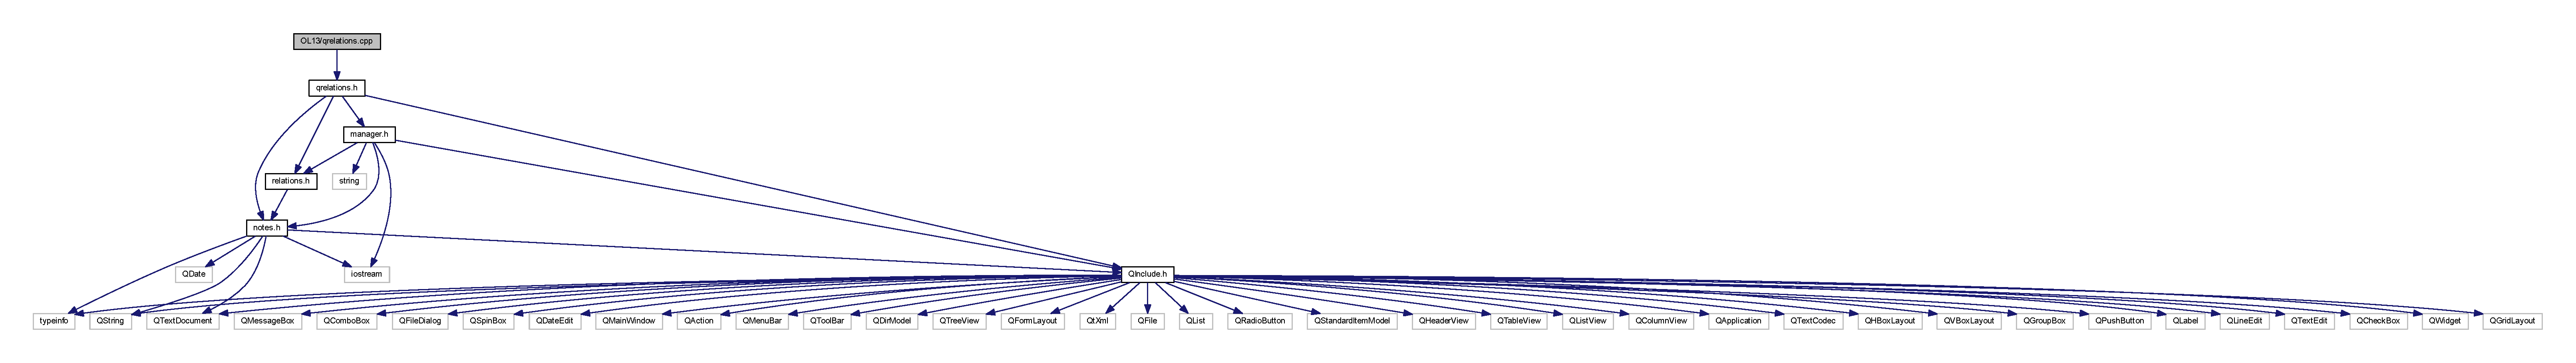
\includegraphics[width=350pt]{qrelations_8cpp__incl}
\end{center}
\end{figure}


\subsection{Detailed Description}
Implémentation des relations de manière graphique. 

\begin{DoxyAuthor}{Author}
Garnier Maxime, Naudin Louise, Pépin Hugues 
\end{DoxyAuthor}
\begin{DoxyVersion}{Version}
1.\+0 
\end{DoxyVersion}
\begin{DoxyDate}{Date}
14 Juin 2017
\end{DoxyDate}
class \+: -\/\+Q\+Dock\+Relation Permet l\textquotesingle{}affichage de la structure arborescente des relations -\/\+Edit\+\_\+\+Notes\+Couples Permet l\textquotesingle{}edition de nouveaux couples -\/\+Edit\+\_\+relation Permet l\textquotesingle{}edition d\textquotesingle{}une nouvelle relation 